\chapter{二类问题实验评估}\label{sec:experiments}
\section{前言}
在第\ref{sec:method}章中,本文详细介绍了所提出模型的结构、背后的原理、损失函数等内容。
\section{数据集介绍}
\subsection{视网膜糖尿病性病变数据集}
\subsection{模拟皮肤病病变数据集}
\section{实验设置}
\section{消融实验:生成器和判别器角色探究}
\begin{figure}[h]
	\centering
	\includegraphics[width=1.0\textwidth]{figure/u_d_c_comparation.pdf}
	\caption{} 
	\label{fig:u_d_c_comparation}
\end{figure}
\begin{figure}[h]
	\centering
	\includegraphics[width=1.0\textwidth]{figure/pr_cureve_u_d_u_c_u_d_c_components.pdf}
	\caption{} 
	\label{fig:u_d_c_comparation_pr_curve}
\end{figure}
\section{在视网膜糖尿病性病变数据集上的实验结果分析}


\begin{figure}[h]
	\centering
	\includegraphics[width=1.0\textwidth]{figure/retinal_image_res.pdf}
	\caption{} 
	\label{fig:retinal_image_res}
\end{figure}


\begin{figure}[h]
	\centering
	\includegraphics[width=1.0\textwidth]{figure/pr_curve_retinal_image/pr_curve.eps}
	\caption{} 
	\label{fig:retinal_image_pr_curve}
\end{figure}
\section{在模拟皮肤病病变数据集上的实验结果分析}

\begin{figure}[h]
	\centering
	\includegraphics[width=1.0\textwidth]{figure/pr_curve_skin_image.pdf}
	\caption{} 
	\label{fig:simulated_skin}
\end{figure}


\begin{figure}[h]
	\centering
	\includegraphics[width=1.0\textwidth]{figure/pr_curve_skin_image/pr_curve.eps}
	\caption{}
	\label{fig:simulated_skin_pr_curve}
\end{figure}
\section{本章小结}



